\chapter{Methodology}
\section{Proposal}
Based on research into RAG vulnerabilities, there is a clear lack of security measures designed to preserve the privacy of a RAG corpus. This is especially important in fields like healthcare.
As demonstrated in \autocite{zeng2024goodbadexploringprivacy}, private information can be easily extracted by determined attackers through simple prompt injections.
Given that RAG relies on a set of documents as context, and that this is vulnerable to attacks, I suggest generating synthetic context from this set of documents.
This set of documents could refer to a patient's records, containing information such as their blood pressure, etc.
A separate LLM will analyze the set of records retrieved by the user's query, comparing the two and extracting relevant information.
The LLM will then generate a synthetic record containing all the information needed to answer the query, whilst removing PII at the same time.
This separates the context given to the LLM from the RAG corpus, whilst still ensuring that its response remains contextually relevant.

\section {Implementation}
To design an adequate system that can preserve a patient's privacy, we must first understand the different types of methods associated with this task.

\subsection{Medical Anonymisation}
According to \autocite{Rodriguez_Tuck_Dozier_Lewis_Eldridge_Jackson_Murray_Weir_2022}, the three main methods in preserving medical privacy are Pseudonymisation, De-identification and Anonymisation.
Pseudonymisation refers to the replacement of attributes with pseudonyms. De-identification refers to the removal of PII from patient records.
Anonymisation refers to the distortion of data such that any record lacks individuality.

The method we will be focusing on is the process of anonymisation.
There are two different ways this is achieved.
Recalculation, which involves turning absolute dates into relative representations (such as turning a patient's date of birth into their equivalent age representation), and Perturbation, which involves directly modifying a patient's medical records away from their original form.

\subsection{System Design}

The proposed system design is outlined in figure \ref{fig:SynthLLMRAG}.
The system is similar to figure \ref{fig:RAGexample}, with the inclusion of an intermediary step that passes both the user query as well as the retrieved context documents to a secondary LLM for synthesis.
The secondary LLM is responsible for both information extraction as well as synthetic document generation.
To mimic privacy requirements, a locally run LLM is used here to ensure that the RAG corpus remains air-gapped.
The use of an adequately sized LLM is critical here, and in our case we will be using Mistral's Nemo-12B.
The synthesized document is then returned to the front-facing LLM along with the user's query to generate an appropriate response.

\begin{figure}
	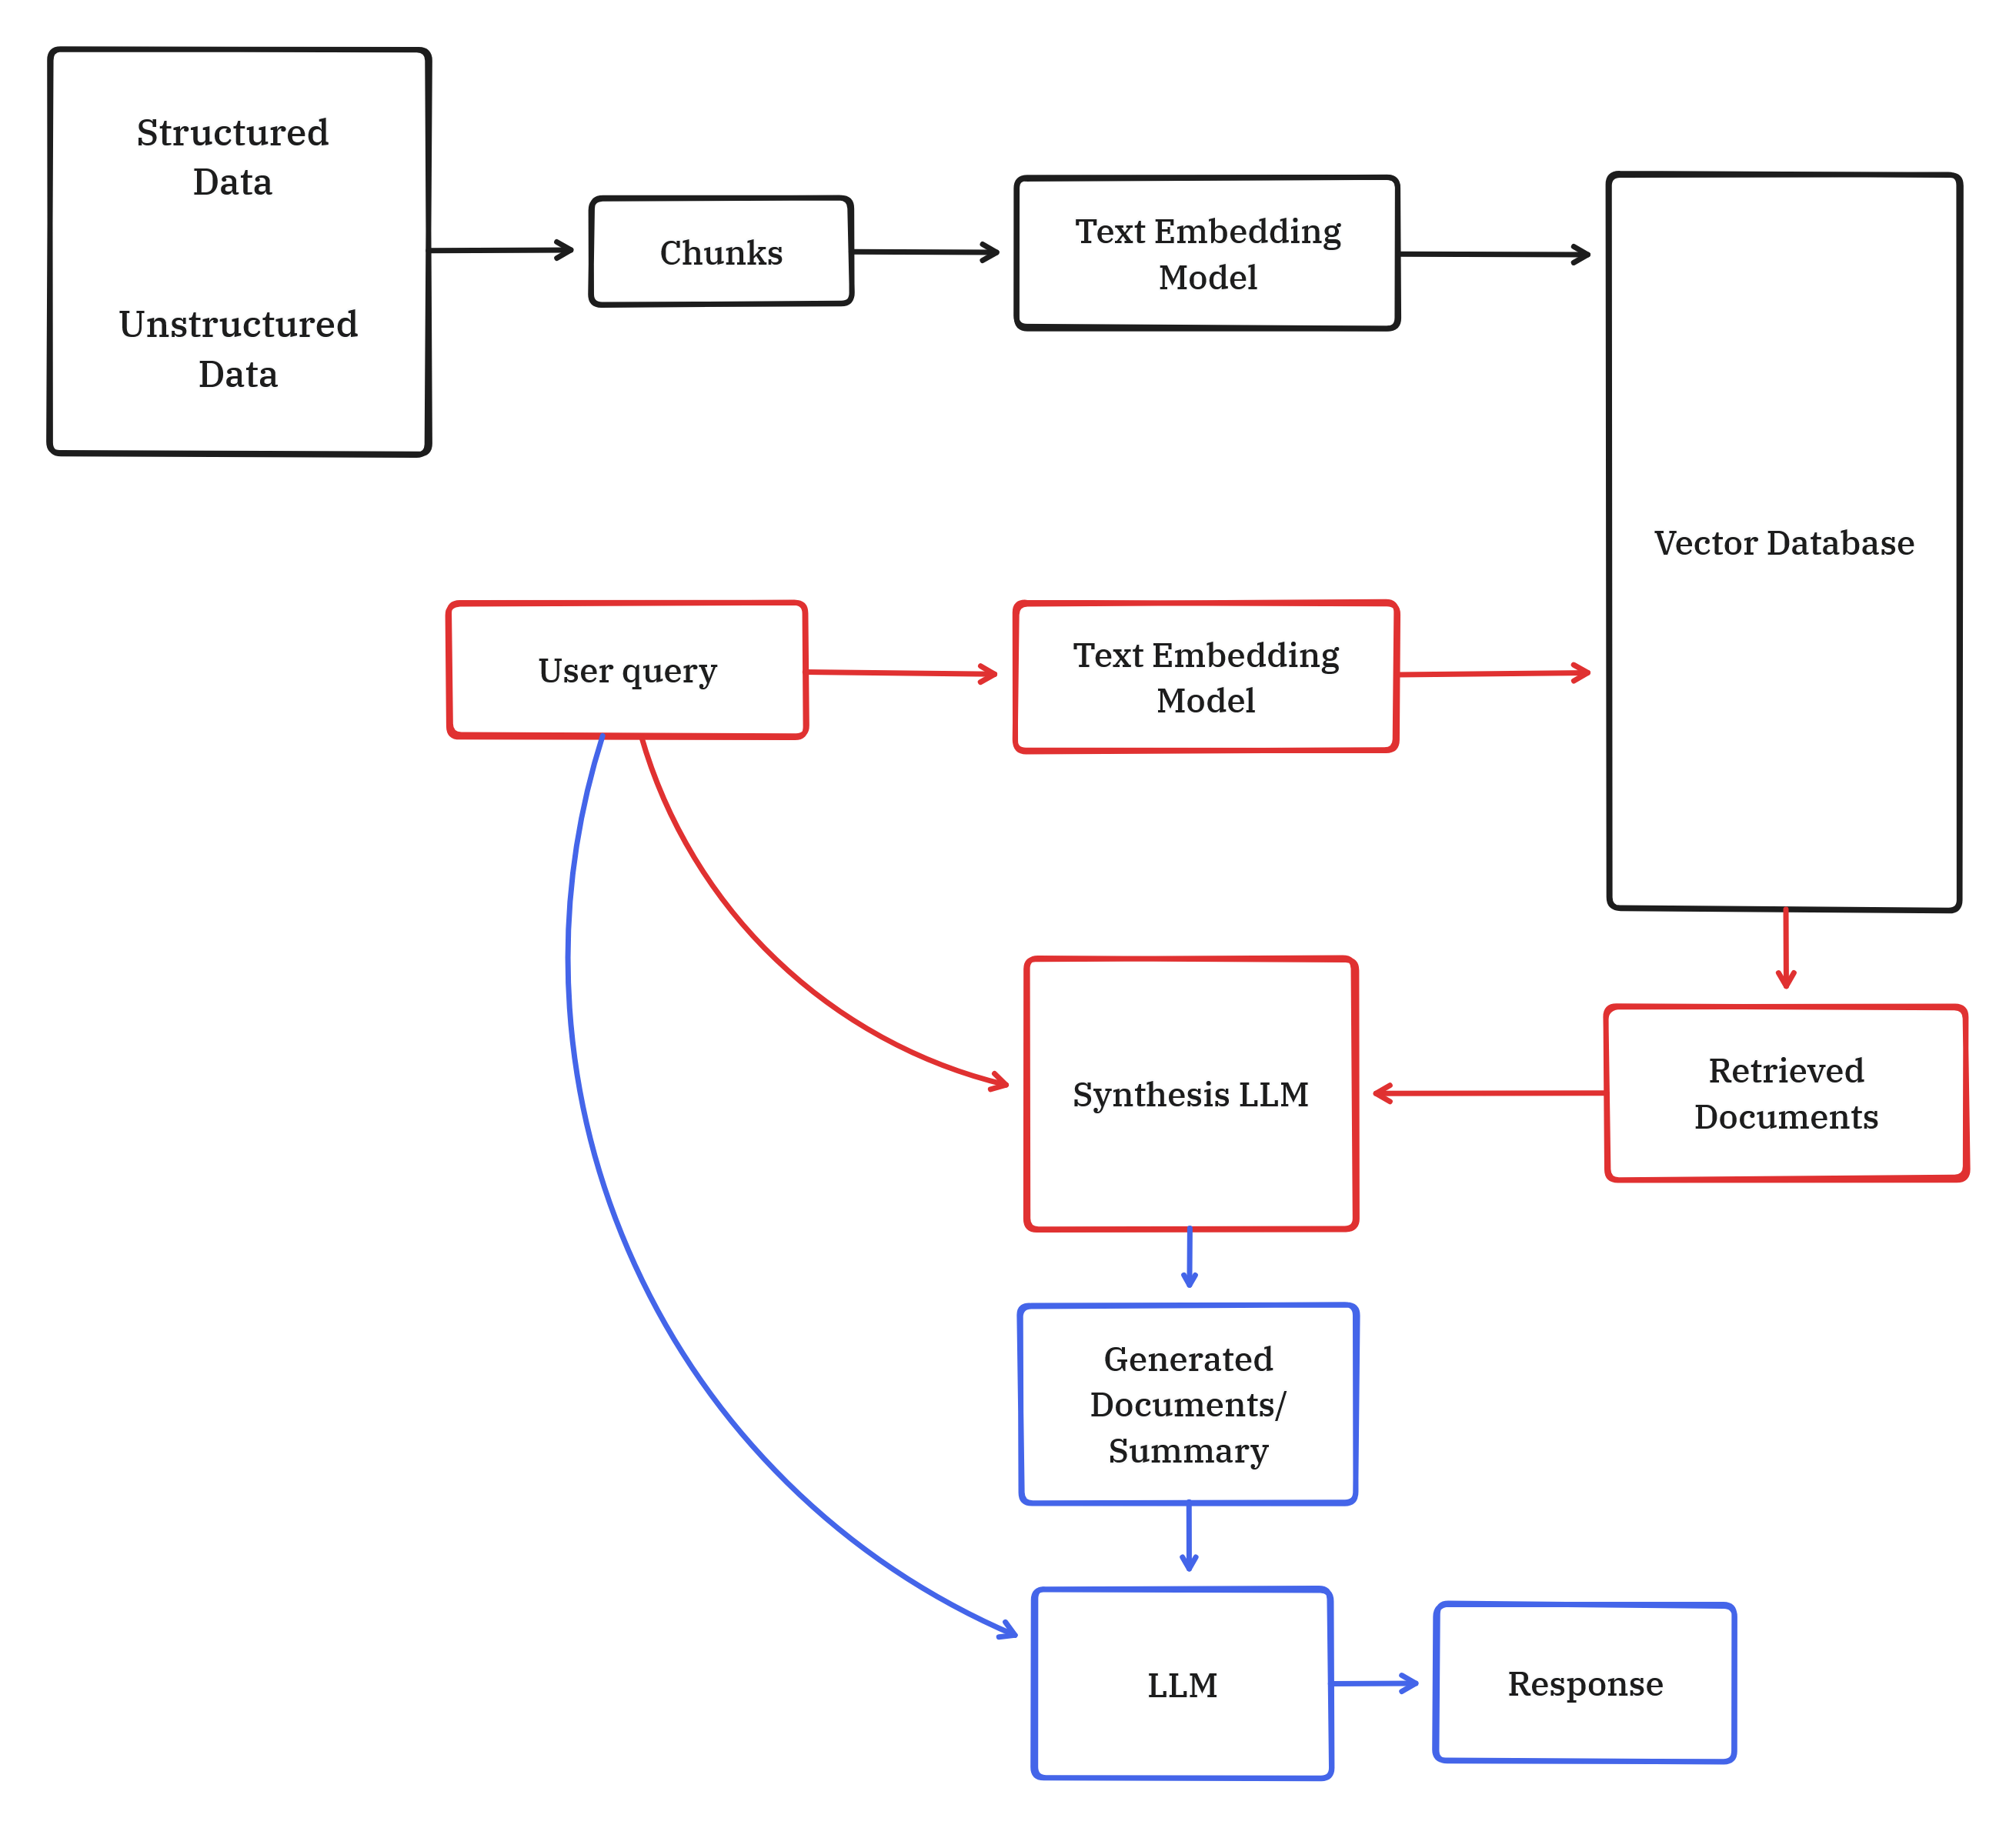
\includegraphics[width=\textwidth]{Synthesis LLM RAG example.png}
	\caption{System Design}
	\centering
	\label{fig:SynthLLMRAG}
\end{figure}

\subsection{Building the RAG Corpus}
RAG systems can make use of either structured or unstructured data.
For our case, we will be making use of a synthetic FHIR dataset, generated by Synthea \autocite{Synthea2024}.
FHIR is a structured healthcare standard that defines how healthcare information can be shared between different systems regardless of how they are stored.
Individual FHIR patient records are stored in what is known as resources.
A resource can take on different types, and each type contains information necessary for its specific use case.
FHIR records can appear in the form of JSON, XML or RDF.
Here we will be making use of JSON FHIR files to create our RAG corpus.

Firstly, we convert FHIR resources to basic sentences.
This is to avoid repeatedly embedding the same key-value token pairs and wasting embedding tokens.
Refer to figure \ref{fig:FHIRtoSentence} for an example.
This can be further truncated.
For example we can simply embed only the name of the reading and its associated value.

\begin{figure}
	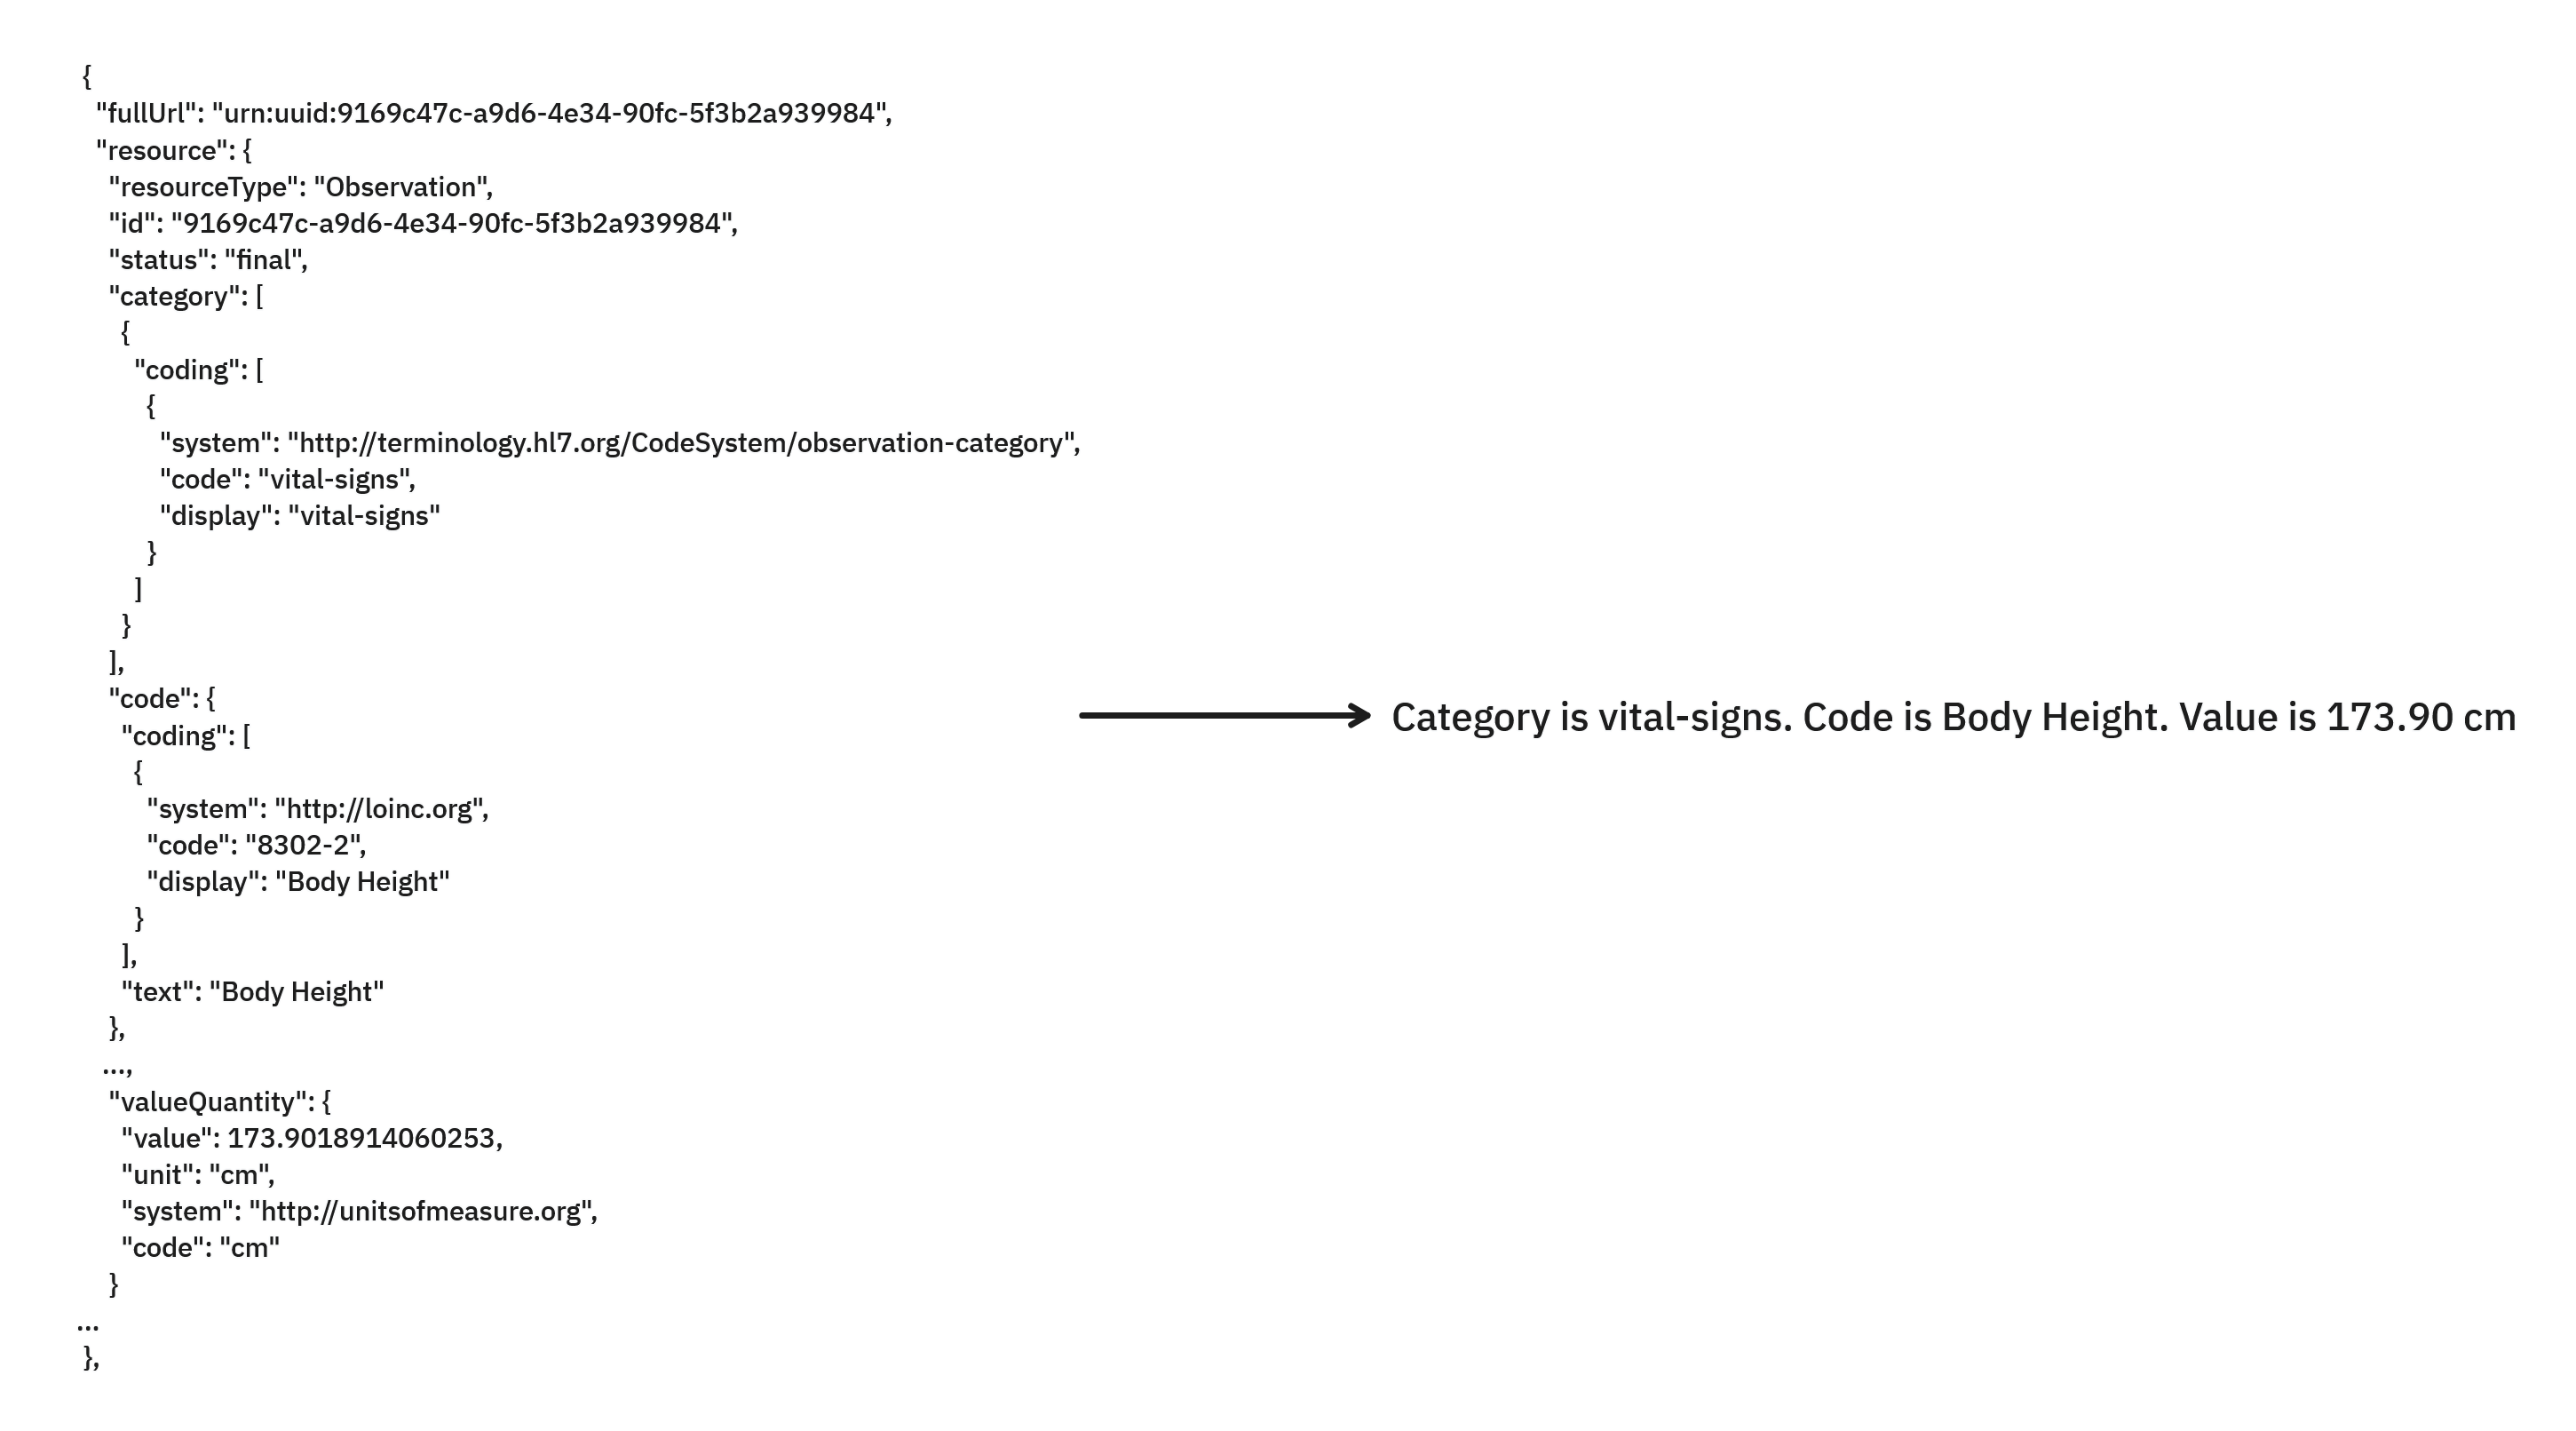
\includegraphics[width=\textwidth]{Converting FHIR to sentence.png}
	\caption{FHIR to sentence}
	\centering
	\label{fig:FHIRtoSentence}
\end{figure}

We perform this operation on the patient's record, extracting Observations and Procedures, separating them by date, and extracting a patient's diagnosed conditions, medications, as well as allergies, and storing them in a separate document.
These documents are then converted into vectors through the use of a text-embedding model.
For this, we will be using the \emph{bge-base-en} embedding model.
The embeddings are then stored in a Postgres database utilizing the \emph{pgvector} extension.

\begin{figure}
	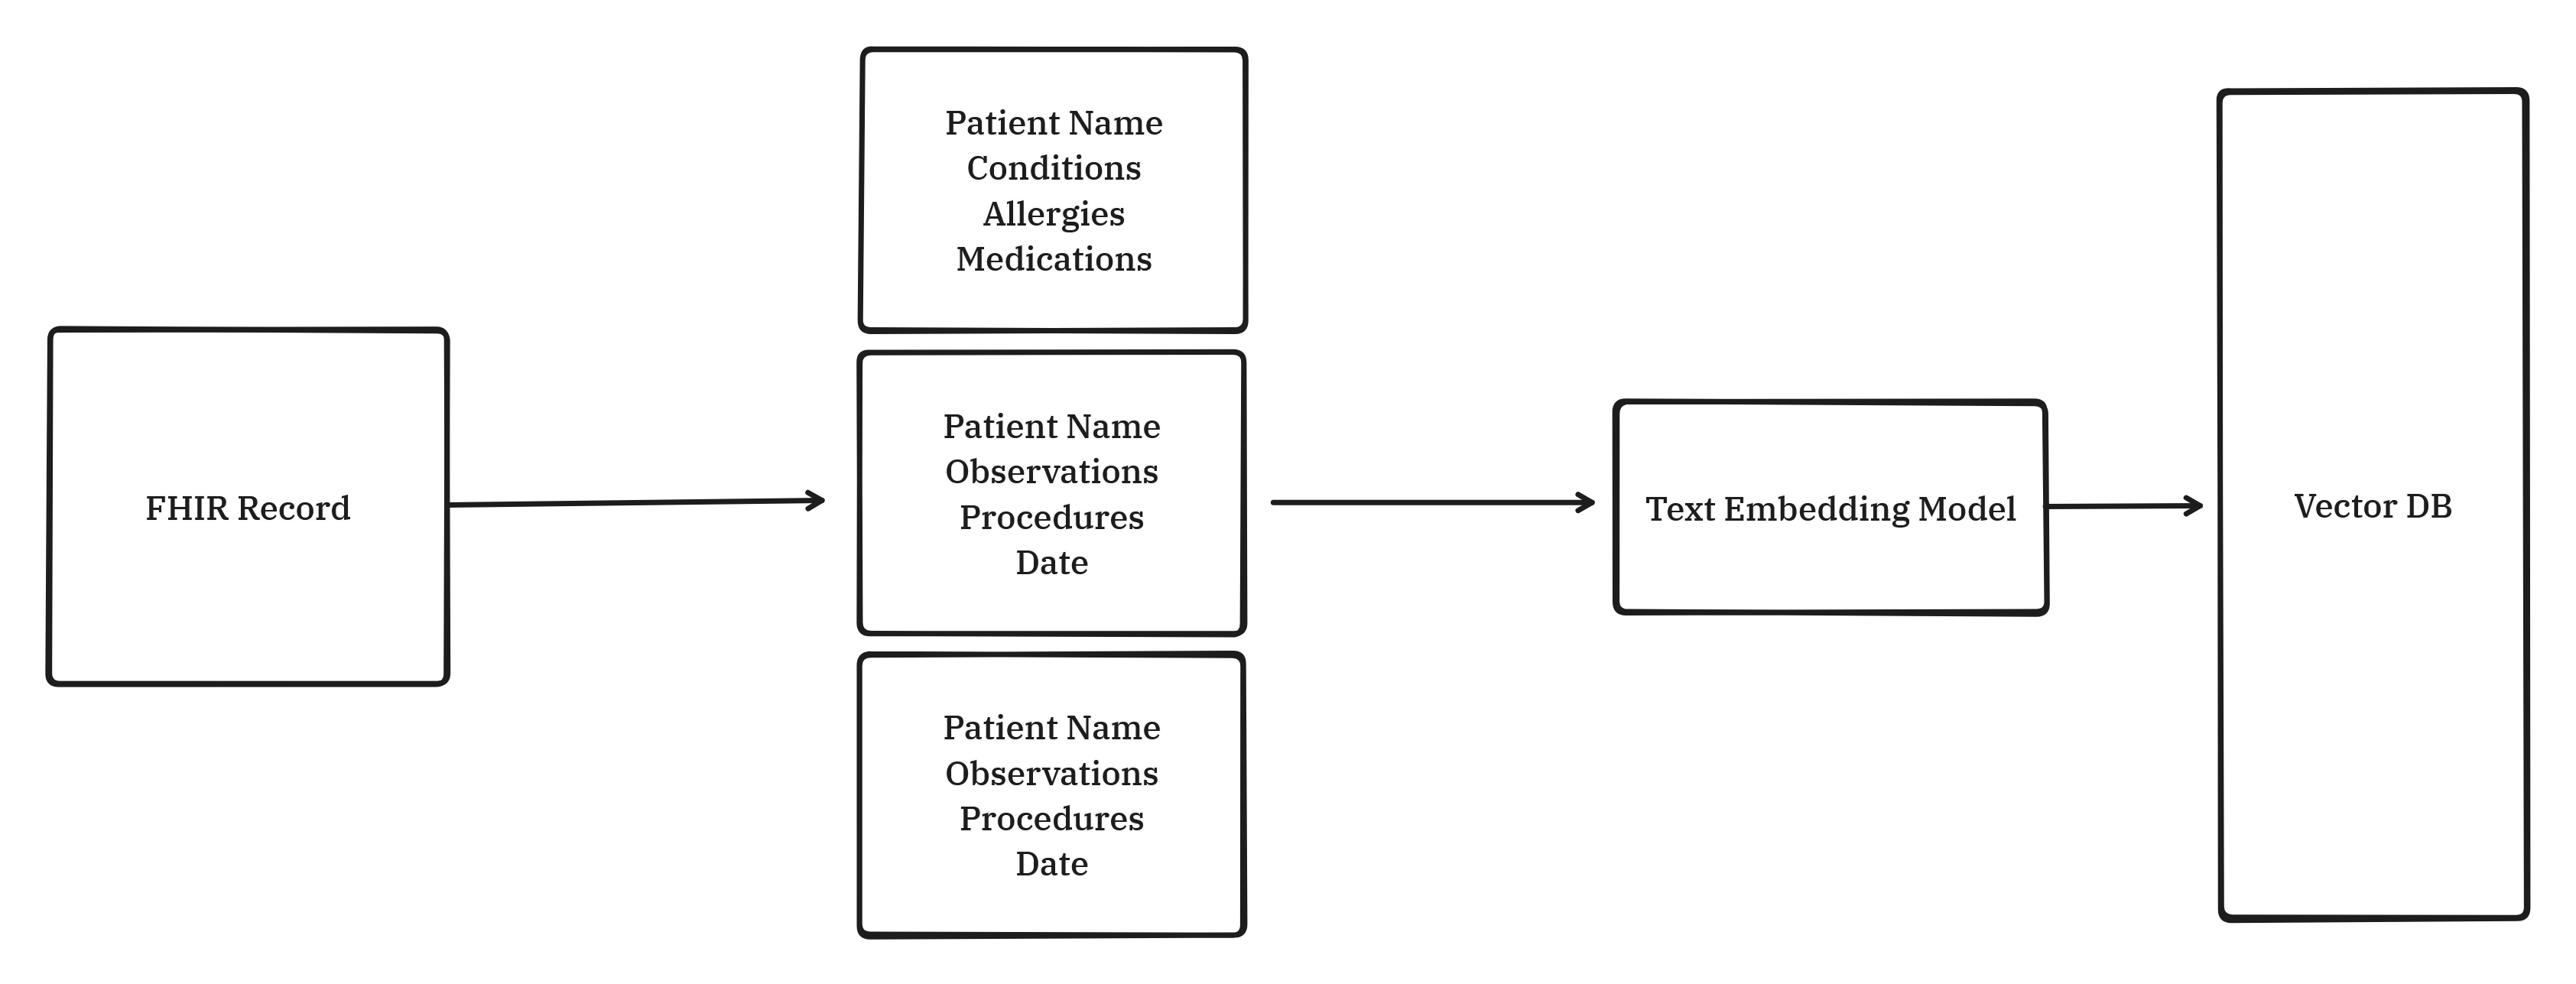
\includegraphics[width=\textwidth]{Store embeddings in DB.png}
	\caption{Embeddings to Database}
	\centering
	\label{fig:EmbeddingsDatabase}
\end{figure}

\subsection{Retrieval}
With the RAG corpus built, we can now move onto retrieving documents associated with a query.
The query goes through the embedding process and its resulting vector is compared to other document vectors in the database.
The top \textit{k} results are returned, with \textit{k} being an adjustable variable.
What determines the chunk's relevance is its cosine similarity to the input query.
Cosine similarity is defined as the following:
\[
	\text{Cosine Similarity} = \cos(\theta) = \frac{\mathbf{A} \cdot \mathbf{B}}{\|\mathbf{A}\| \|\mathbf{B}\|}
\]

and returns a score between 0.0 to 1.0.
Here we can set a minimum cut-off for cosine similarity to adjust the relevance of returned information.
Refer to figure \ref{fig:RetrievalExample} for an example of the returned chunks.

\begin{figure}
	\centering
	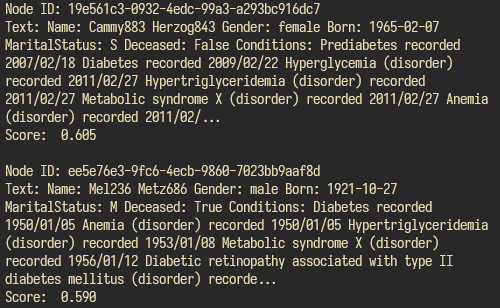
\includegraphics[width=0.5\textwidth]{retrieval example.png}
	\caption{Input Query: Which patients have diabetes?}
	\label{fig:RetrievalExample}
\end{figure}

\subsection{Synthetic Report Generation}
LLMs differ in capabilities in accordance to their size.
To determine if the chosen LLM (Mistral Nemo 12B) was sufficient for what I needed it to do, I tested its summarization and generation abilities.
Firstly, I merged the previously processed FHIR record for a single patient into a combined document.
This document was then passed to LLM along with a set of instructions.
The specific prompt provided to the LLM is in the appendix, but to summarize:
\begin{itemize}
	\item Break the summary into clear sections with headers
	\item Include exact numerical values
	\item Use precise dates
	\item Report conditions with specific terminology
	\item Summarize readings into a range spanning from min-max
\end{itemize}

The generated report summary was then passed to the LLM with instructions to anonymize information by rounding values as well as removing ages, dates, and names.
This was done for three different types of prompting strategies, Zero-Shot, Chain-of-Thought, and Structured Output.

Refer to figure \ref{fig:SynthSummary} for a side-by-side comparison for Zero-Shot generation.
Full results for each are present in the appendix.
Overall, the LLM was effective in following instructions as well as working with a large amount of context.

\begin{figure}
	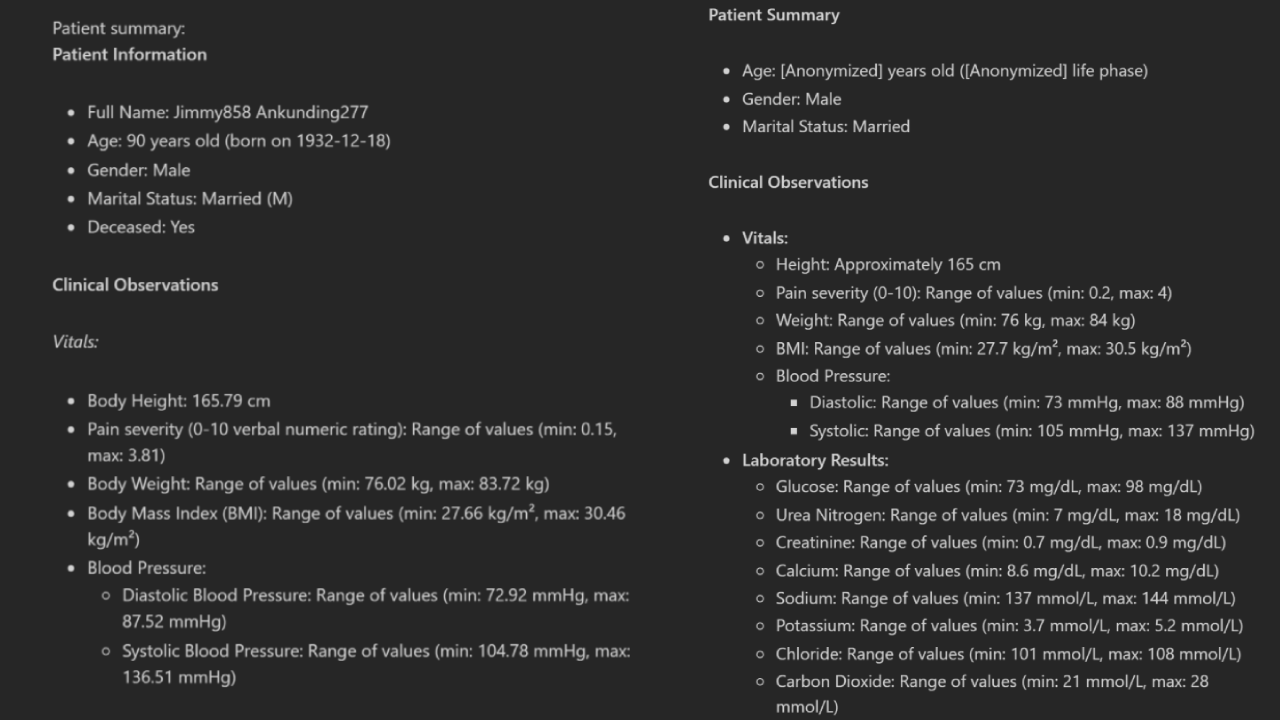
\includegraphics[width=\textwidth]{Zero-shot-summary-vs-synth.png}
	\centering
	\caption{Zero-Shot Generated Summary V.S. Synthesized Summary}
	\label{fig:SynthSummary}
\end{figure}
